The debate on wealth inequality has a long history dating back at least to the work of Kutznets \cite{Kuznets1955} on the U-shaped relationship of inequality on development, where economic growth at first increases wealth inequality and then after a certain point it decreases. Much research has focused on this relation between inequality and growth \cite{PerssonTabellini1994}), and inequality has also been suggested to be positively correlated with a number of indicators of social disfunction, from infant mortality and health to social mobility and crime \cite{TheSpirit}.

\begin{figure}%[htbp]
\centering
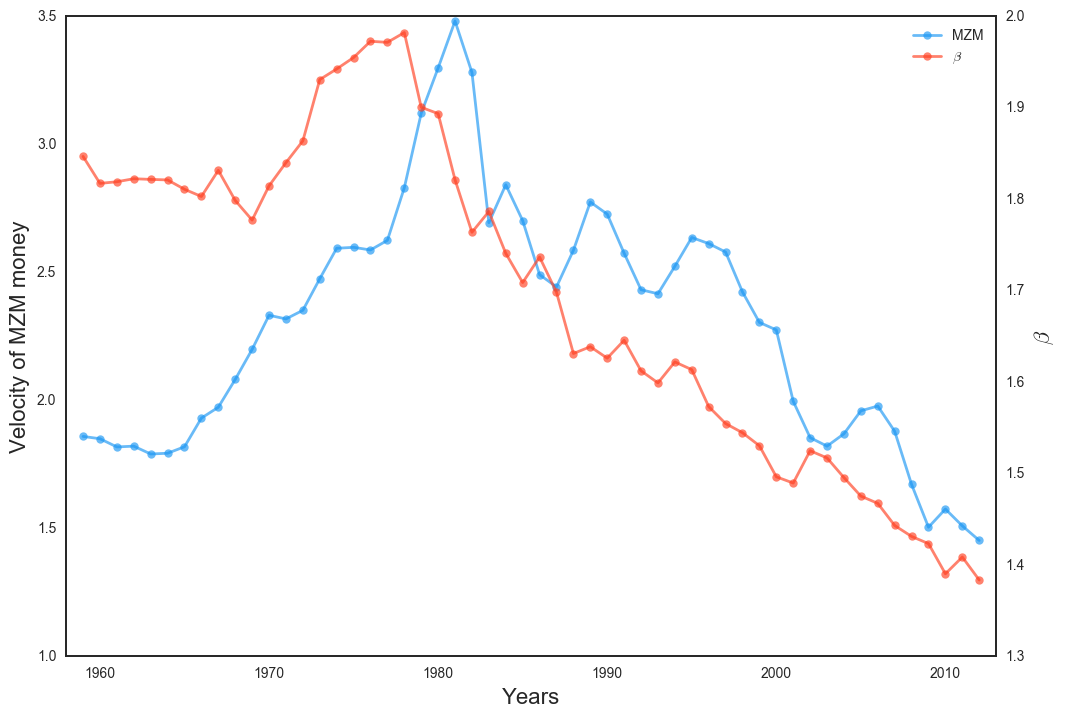
\includegraphics[width=0.59\textwidth]{figs_ineq/data_1.png}
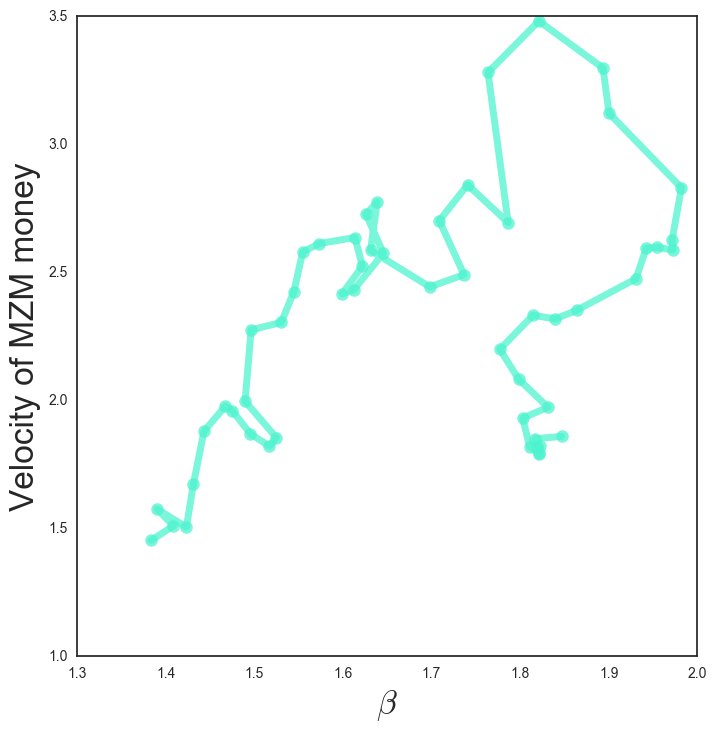
\includegraphics[width=0.39\textwidth]{figs_ineq/data_2.png}
\caption{\textbf{(Left)} Velocity of money of MZM stocks (left y-axis) and Pareto exponent $\beta$ of the wealth distribution (right y-axis) as a function of time. Both time series refer to the US, the data on the money velocity is retrieved from \cite{FRED}, the data on the wealth distribution is taken from \cite{SaezZucman2016}. \textbf{(Right)} MZM velocity of money as a function of $\beta$, for the same data.}
\label{Fig:data}
\end{figure}

The subject has regained much interest recently, in view of the claim that inequality has reached the same levels as in the beginning of the 20th century \cite{Piketty2001}. Saez and Zucman \cite{SaezZucman2016} corroborate these findings, studying the evolution of the distribution of wealth in the US economy over the last century, and they find an increasing concentration of wealth in the hands of the 0.01\% of the richest. Figure \ref{Fig:data} shows that the data in Saez and Zucman \cite{SaezZucman2016} is consistent with a power law distribution $P\{w_i>x\}\sim x^{-\beta}$, with a good agreement down to the 10\% of the richest. The exponent $\beta$ has been steadily decreasing in the last 30 years,  
reaching the same levels it attained at the beginning of the 20th century ($\beta=1.43\pm 0.01$ in 1917).

One of the most robust empirical stylised facts in economics, since the work of Pareto\cite{pareto}, is the observation of a broad distribution of wealth which approximately follows a power law.  What is interesting about it is that such a power law distribution of wealth does not require sophisticated assumptions on the rationality of players as we have dealt so far in this thesis, but it can be reproduced by a plethora of simple models \cite{albert2002, Bouchaud2000, Yakovenko2009Review,Gabaix2009,Sornette2013}, in which it emerges as a typical behaviour within quite general settings. This relates to the often made criticism that the standard approach of Economics, aimed at explaining global behaviour in terms of perfectly rational actors, has largely failed \cite{SMD30,BouchaudCrisis,KirmanBook}. Yet, persistent statistical regularities in empirical data suggest that a less ambitious goal of explaining economic phenomena as emergent statistical properties of a large interacting system may be possible, without requiring much from agents' rationality \cite{Gode1993,Smith2003}. 

Taking inspiration from such independence from economic rationality, our goal is to study inequality via a zero intelligence agent model, in which agents with different capital trade goods randomly in a market. Rather than focusing on the determinants of inequality, we focus on a specific consequence of inequality: its impact on liquidity. There are a number of reasons why this is relevant. First of all, the efficiency of a market economy essentially resides on its ability to allow agents to exchange goods. A direct measure of efficiency is the number of possible exchanges that can be realised or equivalently the probability that a random exchange can take place. This probability quantifies the ``fluidity'' of exchanges and we shall call it \textbf{liquidity} in what follows. This is the primary measure of efficiency that we shall focus on. 

Secondly, liquidity, as intended here, has been the primary concern of monetary polices such as Quantitative Easing aimed at contrasting deflation and the slowing down of the economy, in the aftermath of the 2008 financial crisis. A quantitative measure of liquidity is provided by the \textbf{velocity of money} \cite{IFisher}, measured as the ratio between the nominal Gross Domestic Product and the money stock\footnote{The data reported in this chapter concerns the MZM (money with zero maturity), the broadest definition of money stock that includes all money market funds. We refer to \cite{FRED} for further details.} and it quantifies how often a unit of currency changes hand within the economy. As Figure \ref{Fig:data} shows, the velocity of money has been steadily declining in the last decades, with a clear correlation to the level of inequality. The results in this chapter suggests that the velocity decline and the increasing level of inequality occurring together is not a coincidence. Rather the former is a consequence of the latter. 

Without clear yardsticks marking levels of inequality that seriously hamper the functioning of an economy, the debate on inequality runs the risk of remaining at a qualitative or ideological level. The main finding of the work presented in this chapter is that, in the simplified setting of the model presented, there is a sharp threshold beyond which inequality cripples the economy. More precisely, when the power law exponent of the wealth distribution approaches one, liquidity vanishes and the economy halts because all available (liquid) financial resources concentrate in the hands of few agents. This provides a precise, quantitative measure of when inequality becomes too much. 

The main goal of this work is thus to isolate the relation between inequality and liquidity in the simplest possible model that allows us to draw sharp and robust conclusions. Specifically, the model is based on a simplified trading dynamics in which agents with a Pareto distributed wealth randomly trade goods of different prices.  Agents receive offers to buy goods and each such transaction is executed if it is compatible with the budget constraint of the buying agent. This reflects a situation where, at those prices, agents are indifferent between all feasible allocations. The model is in the spirit of random exchange models, as for example the Statistical Equilibrium of Markets described in Chapter \ref{cha:stat_mech} and in other works \cite{SjurFlam2012, Yakovenko2009Review}, but our emphasis is not on whether the equilibrium can be reached or not. In fact we show that the dynamics converges to a steady state, which corresponds to a maximally entropic state where all feasible allocations occur with the same probability. Rather we focus on the allocation of cash in the resulting stationary state and on the liquidity of the economy, defined as the fraction of attempted exchanges that are successful. Since the wealth distribution is fixed, the causal link between inequality and liquidity is clear in the simplified setting we consider.

In a nutshell, within our model the freezing of the economy occurs because when inequality in the wealth distribution increases, financial resources (i.e. cash) concentrate more and more in the hands of few agents (the wealthiest), leaving the vast majority without the financial means to trade. This ultimately suppresses the probability of successful exchanges, i.e. liquidity. 


\section{The model}
\label{sec:modelDescription}

We introduce an inequality trading model consisting of an economy with $N$ agents, each with wealth $c_i$, $ i = 1, \ldots, N$. There are $M$ objects to be traded among the agents in the economy and each object $m = 1, \ldots,M$ has a price $\pi_m$. A given allocation of goods among the agents is described by an $N\times M$ allocation matrix $\mathcal{A}$ with entries $a_{i,m} = 1$ if agent $i$ owns good $m$ and zero otherwise, but agents can only own baskets of goods they can afford, i.e. whose total value does not exceed their wealth. The wealth of an agent not invested in goods corresponds to the cash (liquid capital) $\ell_i$ that agent $i$ has available for trading, i.e.,

\begin{equation}
c_i -  \sum_{m=1}^M a_{i , m} \pi_m =\ell_i\ge 0, \quad\quad i=1,\ldots,N,
\label{eq:1}
\end{equation}

Therefore the set of feasible allocations -- those for which $\ell_i\ge 0$ for all $i$ -- is only a small fraction of the $M^N$ possible realizations of the allocation matrices $\mathcal{A}$. 

The dynamics are similar to those typical of zero-intelligent agent-based models in economics and are as following: starting from a feasible allocation matrix $\mathcal{A}$, at each time step a good $m$ is picked uniformly at random among all goods. Its owner then attempts to sell it to another agent $i$ also drawn uniformly at random among the other $N-1$ agents. If agent $i$ has enough cash to buy the product $m$, that is if $\ell_i \ge \pi_m$, the transaction is successful and his cash decreases by $\pi_m$ while the cash of the seller increases by $\pi_m$, otherwise the transaction fails, with no possibility of an object being divided. The total capital $c_i$ of agents does not change over time, so $c_i$ and the good prices $\pi_m$ are quenched parameters of the model. We reemphasize that there are no decisions to be made by the agents, they have no utility function to maximize and simply accept trades when selected if they have enough cash.

A crucial property of these dynamical rules is that the stochastic transition matrix $W(\mathcal{A}\to\mathcal{A}')$ is symmetric between any two feasible configurations $\mathcal{A}$ and $\mathcal{A}'$: $W(\mathcal{A}\to \mathcal{A}') = W(\mathcal{A}'\to \mathcal{A})$ and any feasible allocation $\mathcal{A}$ can be reached from any other feasible allocation $\mathcal{A}'$ by a sequence of trades. This implies that the dynamic satisfies the detailed balance condition:

\begin{align}
W(\mathcal{A} \to \mathcal{A}') P(\mathcal{A}) = W(\mathcal{A}'\to \mathcal{A})P(\mathcal{A}'),  \quad \forall \mathcal{A}, \mathcal{A}'
\end{align}
with a stationary distribution over the space of feasible configurations that is uniform, i.e., $P(\mathcal{A})= \frac{1}{A}$, where $A$ is the number of feasible allocations. This is a consequence of the symmetric transition rates, and would be the same for every trading rule that has $W(\mathcal{A}\to \mathcal{A}') = W(\mathcal{A}'\to \mathcal{A})$. In fact, the current trading rules employed in this model are a particular case of a general rule for which we first select a subset of $n$ agents, $2 \leq n \leq N$, then we pick a random good from these $n$ agents and try to trade it with the remaining $n-1$ agents, automatically accepting if the chosen buyer has enough cash to purchase it. This rule may sound cryptic, but it's familiar in the particular cases of $n=N$, which is the current one described in the model, and of $n=2$, in which we first pick two consumers and then try to exchange a random good among themselves. All of these rules generate the same stationary distribution.


For the distribution of agents capital, we focus on realisations where the wealth $c_i$ is drawn from a Pareto distribution $P\{c_i> c\} \sim c^{-\beta}$, for $c>c_{\min}$ for each agent $i$, which is compatible with many empirical observations of real world wealth distribution. The parameter $\beta$ will be the main quantity to be explored in this work because it regulates the different levels of inequality among the agents. To compare different economies, the ratio between the total wealth $C=\sum_i c_i$ and the total value of all objects $\Pi=\sum_{m}\pi_m$ will be kept fixed. Because $C$ is a random variable with potentially very high variance, the number of goods $M$ is realization dependent, we will populate the economy with as many items as needed to keep the ratio $C/\Pi$ constant, which will be described in details late. In order to have feasible allocations, it must hold that $C>\Pi$.

For the goods, we are going to limit the analysis to cases where the $M$ objects are divided into a small number of $K$ classes with $M_k$ objects per class ($k=1,\ldots,K$), where objects belonging to class $k$ have the same price $\pi_{(k)}$. If $z_{i,k}$ is the number of object of class $k$ that agent $i$ owns, then the budget condition given by equation \eqref{eq:1} takes the form

\begin{equation}
c_i =  \sum_{k=1}^K z_{i , k} \pi_{(k)} + \ell_i
\end{equation}

As with standard Statistical Mechanics systems, we will throughout this work assume that the economy is very large, that is, $N, M \to \infty$ but with the ratio $C/\Pi$ constant. This will allow us to calculate the probability distribution of goods $P (z_i^k | c_i)$ for each agent in an exact manner in the large system (thermodynamic) limit. In the next section we will solve the master equation and find the distribution of goods as a function of capital $c_i$. As it will be shown, the main result of this model is that the flow of goods among agents becomes more and more congested as inequality increases until it halts completely when the Pareto exponent $\beta$ tends to one.


\section{The case of one type of good}

We begin our analysis by the simplest case in which there is only one type of good being traded, i.e., $K=1$ with prices $\pi_k = \pi$, but the results shown will extend for the general setting. A formal approach to this problem would consist in writing the complete master equation that describes the evolution for the probability $P(z_1,\ldots, z_N)$ of finding the economy in a state where each agent $i=1,\ldots,N$ has a specific number $z_i$ of goods. We would then take the sum over all values of $z_j$ for $j\neq i$ to derive the master equation for a single agent with wealth $c_i$. However, due to the mean-field like nature of the interactions, we can directly write the detailed balance conditions for a single marginal $P_i(z)$, which will be solvable with a few approximations that exploit the large system size. The detailed balance equation for a single agent is

\begin{align}
\label{eq:full_master_equation_k1}
\Delta P_i(z) & =  P_i(z+1 \to z) P_i(z+1) + P_i(z-1 \to z) P_i(z-1) \\
& - \left(P_i(z \to z + 1) P_i(z) + P_i(z \to z - 1) P_i(z) \right)
\end{align}

However, there are further steps we can take to simplify this equation: we are looking for the stationary distribution of $P_i(z)$ knowing that all the feasible allocations $\mathcal{A}$ are equiprobable and the probability rates are symmetric, $W(\mathcal{A}\to \mathcal{A}') = W(\mathcal{A}'\to \mathcal{A})$. We therefore can solve the detailed balance equation using a stronger condition in which, not only it has to hold that the probability of coming to a state $z$ has to be equal to the probability of leaving it, as equation \eqref{eq:full_master_equation_k1} states, but instead requiring that the probability of going from a specific state $z$ to another $z'$ is equal to the probability of going from $z'$ to $z$. If we take $z' = z + 1$, we have

\begin{equation}
P_i(z + 1) P_i(z + 1 \to z) = P_i(z) P(z \to z + 1)
\end{equation}

The transition probabilities are given as follows: $P_i(z + 1 \to z)$ is the probability of selling a good, which is composed of two independent events: \emph{(i)} a good of agent $i$ is chosen as the good to be traded, which happens with probability $\frac{z+1}{M}$ and \emph{(ii)} the transaction is successful, ie, the chosen recipient is able to afford the good. This happens with probability $p^s$, whose form we will write later. Therefore $P_i(z + 1 \to z)$ is given by $\frac{z+1}{M}  p^s$. $P_i(z \to z+1)$, on the other hand, is the probability that agent $i$ buys a good, which happens if a good he doesn't own is chosen, which has probability $\frac{M - z}{M}$, he is picked as buyer, with probability $\frac{1}{N-1}$ and has enough cash to purchase it. This means the probability is truncated by a term $1-\delta_{z, m_{i}}$, where $m_{i}=\floor{c_i / \pi}$ is the maximum number of goods which agent $i$ can buy with his wealth $c_i$. If $z=m_{i}$ then he cannot afford the item and the probability is zero.

We put it all together and make two large size approximations: $\frac{1}{N-1} \approx \frac{1}{N}$ and $\frac{M -z}{M} \approx 1$, that is, we used the fact that $N \gg 1$ and $z \ll M$. The first assumption holds by definition, but the latter breaks down if $\beta < 1$, as we will discuss later. We finally have the simplified detailed balance equation for agent $i$


\begin{equation}
P_i(z+1)  \frac{z+1}{M}  p^s =  P_i(z) \frac{1}{N} \left(1-\delta_{z, m_{i}}\right) ,\qquad z=0,1,\ldots, m_i
\label{eq:master_equation_simple_k1}
\end{equation}

The probability of success $p^s$ for the trade is given by

\begin{align}
p^s & =  1-\frac{1}{N-1}\sum_{j\neq i} P(z_j=m_j|z_i=z) \\
 & \cong  1-\frac{1}{N}\sum_{j} P_j(m_j)\qquad (N,M\gg 1)
\label{eq:ps_1Guy}
\end{align}
where the last relation holds because when $N,M\gg 1$ the dependence on $z$ and on agent $i$ becomes negligible. This is important because it implies that for large $N$ the variables $z_i$ can be considered as independent, i.e., $P(z_1,\ldots, z_N)=\prod_i P_i(z_i)$, and the problem can be reduced to that of computing properties from the marginals $P_i(z)$. The probability $p^s$ will be the main dynamical quantity of interest in this model, as an indicator of market activity: when $p^s$ is close to 1, all trades succeed and we consider the market liquid, with goods trading hand frequently. When $p^s \to 0$, most transactions fail and the market becomes frozen.

We can plug an Ansatz in equation \eqref{eq:master_equation_simple_k1} and see that it is solved by a truncated Poisson distribution with parameter $\lambda = M / (N p^s)$:

\begin{equation}
P_i(z) = \frac{1}{Z_i} \left( \frac{\lambda^{z}}{z!}\right) \Theta\left(m_i - z \right),
\label{Eq:ME_solution_1Good}
\end{equation}
where $Z_i$ is a normalization factor that can be determined by $\sum_{z} P_i(z) = 1$. The value of $p^s$, or equivalently of $\lambda$, can be found only in certain approximations of equation \eqref{eq:ps_1Guy}, which we will show later.


%%%% TWO CLASSES OF AGENTS
From the stationary distribution \eqref{Eq:ME_solution_1Good}, we see that the most likely value of $z$ for an agent with $m_i=m$ is given by

\begin{equation}
z^\ast(m)  = \argmax_z  P(z)=
\begin{cases}
    m, & \text{ if } m \leq \lambda \\
    \lambda, & \text{ if } m \geq \lambda
  \end{cases}.
  \label{Eq:cases_ztyp}
\end{equation}

\begin{figure}%[htbp!]
\centering
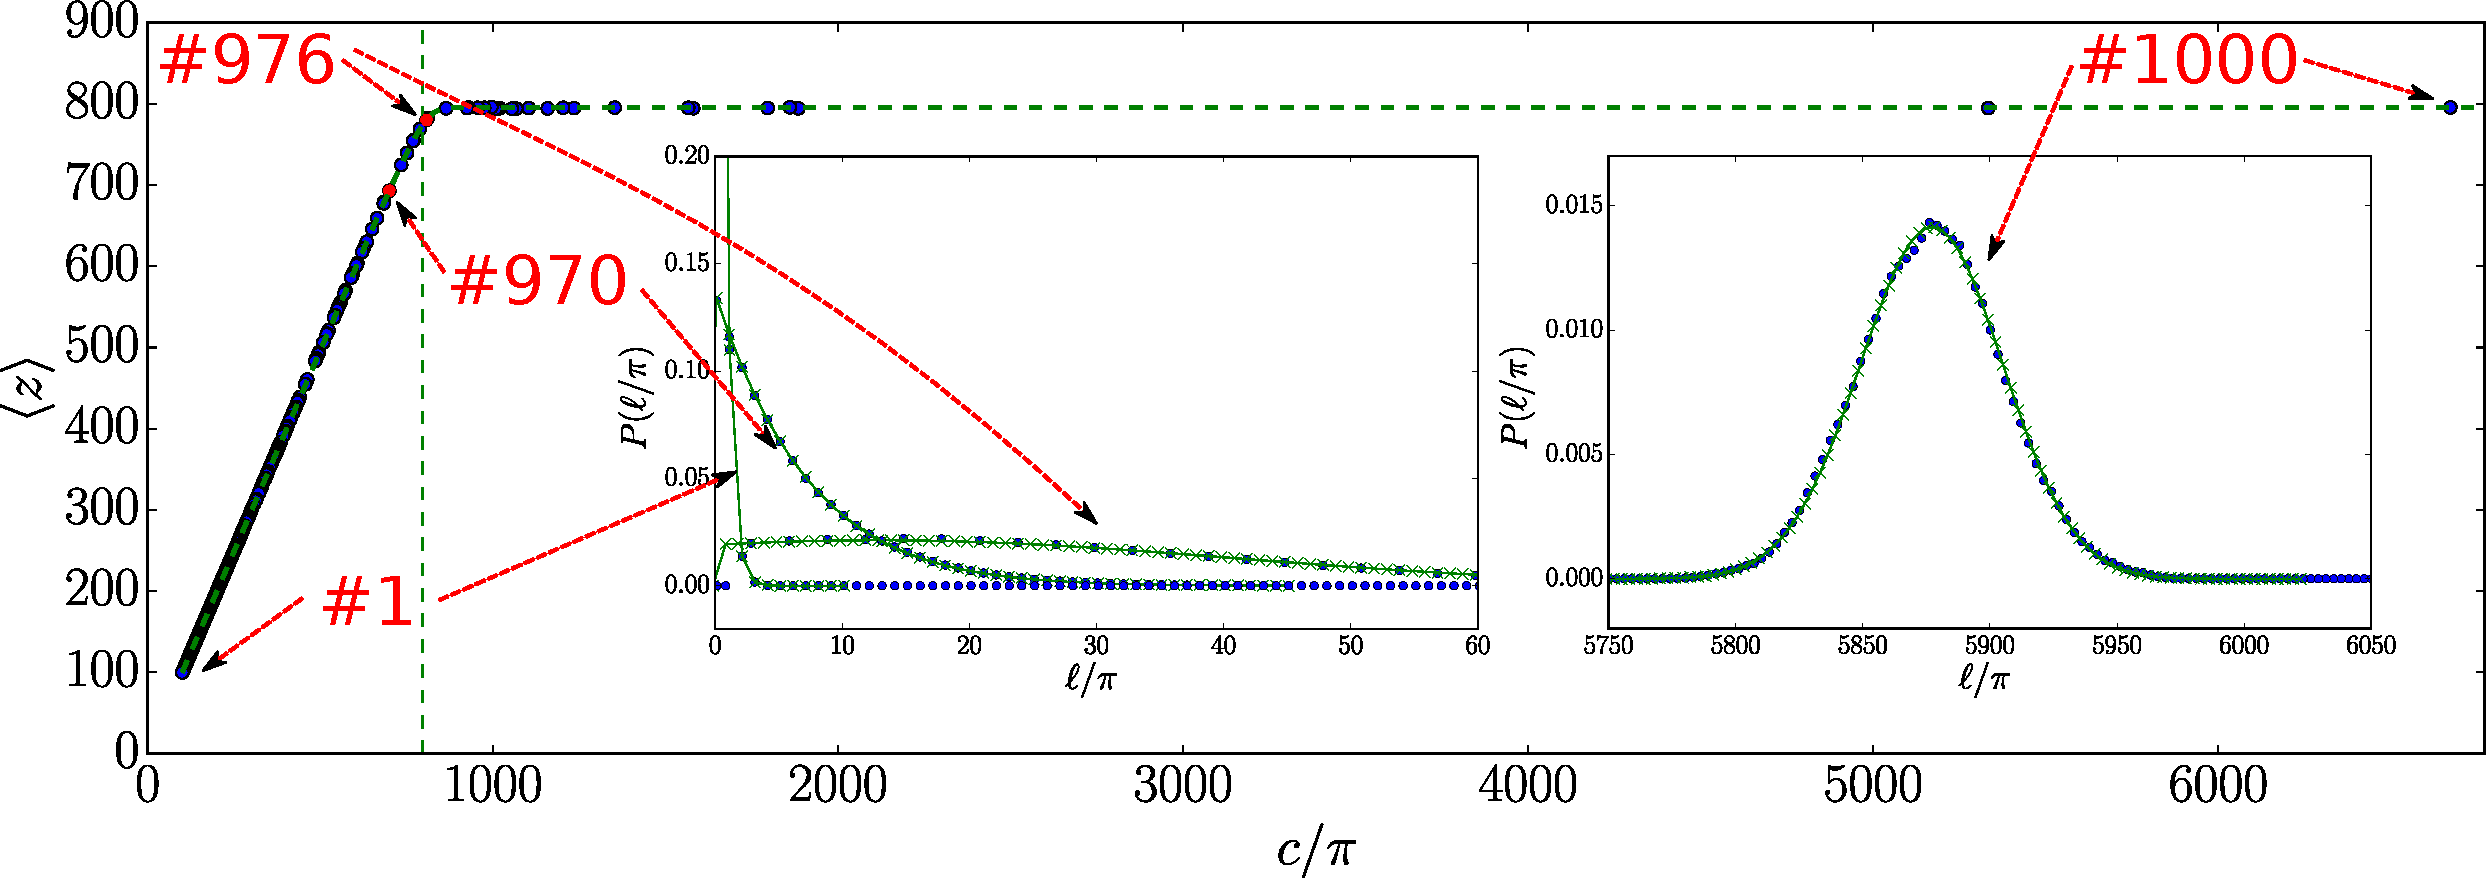
\includegraphics[width=\textwidth]{figs_ineq/fig3_ownership_average_beta=1p80_e=1p10-byHand.pdf}
\caption{\textbf{(Main)} Average number of owned goods in an economy with a single type of good, $N=10^3$ agents, $\beta=1.8$, $M\approx 2 . 10^5$ and $C/\Pi=1.1$. Points $\{(\langle z \rangle_i,c_i)\}_{i=1}^{N}$ denote the average composition of capital for different agents obtained in Monte Carlo simulations, compared with the analytical solution obtained from the Master Equation (green dashed line) given by equation \eqref{Eq:ME_solution_1Good}. The vertical dashed line at $c^{(1)}\simeq 7.98=M/N p^s_1$ indicates the analytically predicted value of the crossover wealth that separates the two classes of agents. \textbf{(Insets)} Cash distributions $P_i(\ell)$ for indicated agents. Agent $\#1$ is the poorest and has very high probability of owning few (around $z_i = 3$) goods, which quickly goes to zero at $z_i = 5$ goods. Agents $\#970$ and $\#976$ are near the class threshold and have reasonable probability of having several goods. Agent $\#1000$ is the richest of the simulation and has two orders of magnitude more goods, with no probability of having less than a hundred times more than agent $\#976$.}
\label{Fig:Picturesque_RichPoor_transition_beta}
\end{figure}

This provides a natural distinction between cash-poor agents -- those with $m \leq \lambda$ --  that often cannot afford to buy any other object, and cash-rich ones -- those with $m> \lambda$ --  who typically have enough cash to buy further objects. We can run computer simulations for the model and compare the goods distribution after equilibrium against theoretical predictions, the results are shown in figure \ref{Fig:Picturesque_RichPoor_transition_beta}. We indeed observe these two types of agents in the simulations, which agree very well with the prediction. The inset shows the cash distribution $P_i(\ell/\pi)$ (where $\ell/\pi = c_i/\pi - z$ represents the number of goods they are able to buy) for some representative agents. While cash-poor agents have a cash distribution peaked at $0$, the wealthiest agents have cash in abundance. When $\lambda\gg 1$, the distribution $P_i(z)$ is sharply peaked around $z^{\text{mode}}(m)$ so that its average is $\langle z\rangle\simeq z^{\text{mode}}(m)$. Then the separation between the two classes becomes rather sharp, as it is the case for Figure \ref{Fig:Picturesque_RichPoor_transition_beta}.

In terms of wealth, we can use the threshold shown in equation \eqref{Eq:cases_ztyp} to define the threshold wealth $c^{(1)}$ for which the poor are defined as those with $c_i<c^{(1)}$ whereas the rich ones have $c_i>c^{(1)}$. This threshold wealth is given by the initial capital an agent requires to have $m = \lambda$. Because all goods have the same price, this is simply given by $\lambda \pi$. So the threshold wealth for the two classes $c^{(1)}$ is given by

\begin{equation}
c^{(1)} = \lambda \pi = M \pi/(N p^s)
\label{eq:c1}
\end{equation}

We can compute $p^s$ by using equation \eqref{eq:ps_1Guy}, $p^s = 1 - \frac{1}{N} \sum_{i=1}^{N} P_i(z = m_i)$, and approximating the probability to be on a threshold $P_i(z=m_i)$ by

\begin{align}
P_i(z=m_i) = 
\begin{cases}
\left( 1 - \frac{m_i}{\lambda} \right) & \text{ for } m_i \ll \lambda \\
0 & \text{ for } m_i > \lambda
\end{cases}
\label{eq:k1_saturated_prob}
\end{align}

The first case can be understood by noting that in the limit $m_i \ll \lambda$ we have the approximation

\begin{equation}
\label{eq:ps_analytical_series}
P_i(z=m_i) = \frac{\lambda^{m_i} \frac{1}{m_i!}}{\sum_{x=0}^{m_i} \lambda^x \frac{1}{x!}} = \frac{1}{1 + \frac{m_i}{\lambda} + \frac{m_i (m_i -1)}{\lambda^2} + \ldots} \simeq  \left( 1 - \frac{m_i}{\lambda} \right),
\end{equation}

Assuming this approximation to be valid for all $m_i < \lambda$ is clearly a bad assumption for all agents with $m_i$ close to $\lambda$. However the wealth is power law distributed and so the weight of agents with $m_i \sim \lambda$ is negligible in the sum over all agents in equation \eqref{eq:ps_analytical_series}. The accuracy of this approximation increases when the exponent of the power law $\beta$ decreases and the mass of agents with capitals around $\lambda$ vanquishes. 

We use equation \eqref{eq:k1_saturated_prob} and write $m_i \approx \frac{c_i}{\pi}$ to rewrite equation \eqref{eq:ps_1Guy}:

\begin{equation}
\label{eq:ps_first_approx}
p^s = 1 - \frac{1}{N} \sum_{i=1}^{N} P_i(z = m_i) \simeq 1 - \frac{1}{N} \sum_{i=1}^N \left(1 - \frac{c_i}{\lambda \pi}\right) \Theta\left(c_i - \lambda \pi \right)
\end{equation}

Because we have a very large number of agents, we are able to transform the sum over the agents into an integral over the capital $c$, with density equal to the capital distribution, ie, we replace

\begin{equation}
\frac{1}{N} \sum_i c_i \to \int_1^\infty c \beta c^{-\beta - 1} dc
\end{equation}

Thus when we truncate by $c_i \leq \lambda \pi = c^{(1)}$ we get

\begin{equation}
\label{eq:app_ps_analytic1}
p^s = 1 - \int_1^{c^{(1)} = \lambda \pi} dc\, \beta c^{-\beta - 1} \left( 1 - \frac{c}{\lambda \pi} \right).
\end{equation}

This is an implicit expression for $p^s$, since it appears on the left hand side of the equation and also inside the integral, because $\lambda = \frac{M}{N p^s}$, which makes it intractable to solve analytically. 

However, we can get good insights on the behavior of $p^s$ by again exploiting the fact that we are assuming a very large system and take $N, M \to \infty$. In this limit, $\lambda$ can be replaced by its expected value on the realizations, i.e., for finite system sizes, $M/N$ is a random variable that depends on the realization of the capital distribution due to the fixed constant $\Pi/C$, but in the limit we can replace $M$ by it's expected value, $\Pi/\pi$ and $N$ by $C / \langle c \rangle$, where $\langle c \rangle$ is the expected capital per agent, which is given by the average of the beta distribution, $\langle c \rangle = \beta/(\beta-1)$. For finite $N$, this is only a reasonable approximation if $\beta \gg 1$, and breaks down in the limit $\beta \to 1^+$ due to the infinite variance of the capital distribution, but it should be accurate for all $\beta > 1$ in the limit $N \to \infty$. Using the approximation on \eqref{eq:c1} and replacing $\lambda = c^{(1)} / \pi$, we have:

\begin{equation}
\frac{M}{N \lambda} \to \left \langle \frac{M}{N} \right \rangle \frac{\pi}{c^{(1)}} = \frac{\Pi}{C} \frac{\beta}{\beta - 1} \frac{1}{c^{(1)}}
\end{equation}

So the equation for $p^s$ is, by the definition of $\lambda$:

\begin{equation}
 \label{Eq:ps_correct}
p^s = \frac{M}{N \lambda} = \frac{\Pi}{C} \frac{\langle c \rangle}{c^{(1)}},
\end{equation} 
which gives us $p^s$ but as a function of $c^{(1)}$, which we still don't know. But now that this is independent of $p^s$, we can put this expression back into \eqref{eq:app_ps_analytic1} and carry out the integration to get an analytic form for $c^{(1)}$:

\begin{equation}
\frac{\Pi}{C} \frac{\langle c \rangle}{c^{(1)}} = {c^{(1)}}^{-\beta} \left( \frac{1}{1-\beta} \right) - \frac{\beta}{1 - \beta } \frac{1}{c^{(1)}},
\end{equation}

Solving for $c^{(1)}$ we have

\begin{equation}
\label{Eq:c1_correct}
c^{(1)} = \left[\beta \left(  1 - \frac{\Pi}{C}\right) \right]^{1/(1 - \beta)}.
\end{equation}

And replacing this back on equation \eqref{Eq:ps_correct} gives $p_s$ as a function of the intensive variables for the economy

\begin{equation}
\label{eq:ps_1good_final}
p^s = \frac{\Pi}{C}\frac{\beta}{\beta - 1} \frac{1}{\left[\beta \left(1 - \frac{\Pi}{C}\right) \right]^{1/(1 - \beta)}}.
\end{equation}

\begin{figure}[!ht]
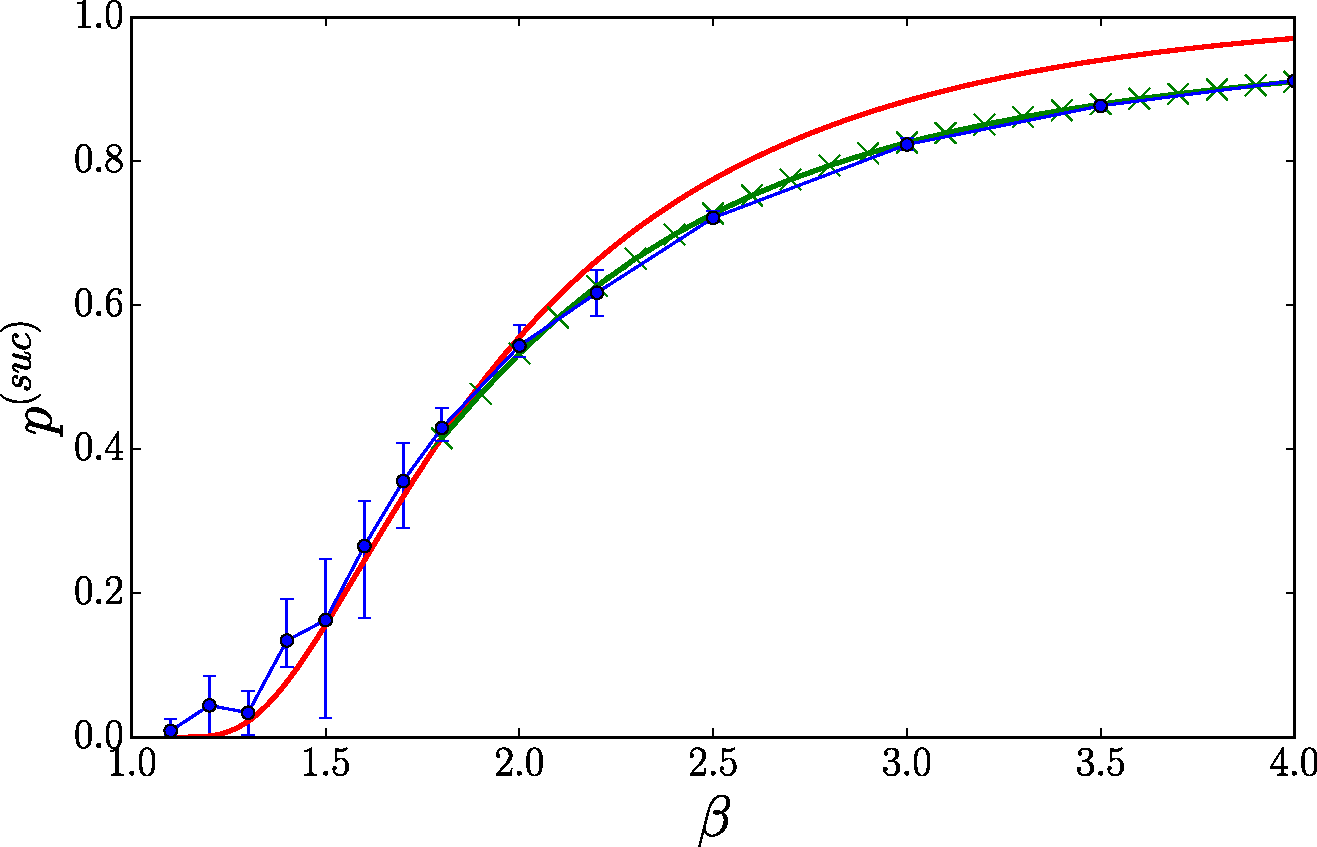
\includegraphics[width=\textwidth]{figs_ineq/fig_K=1_e=1p2_g=undef_ps_prediction_unadj.pdf}
\caption{Comparison between numerical simulations and analytical estimates for the success probability of transaction $p^s$ for one class of goods, as a function of the Pareto exponent $\beta$. The blue solid circles are the result  of Monte Carlo simulations performed for $N=10^5$ agents and averaged over 5 realizations, with the error bars indicating the min and max value of $p^s$ over all realizations. The red lines are the analytic estimates  according to equation \eqref{eq:ps_1good_final}. The green crossed lines correspond to numerically iterating equation  \eqref{eq:ps_first_approx} for a population composed of $N=64$ "agents". For lower $\beta$ the capital distribution becomes too broad and this solution becomes unfeasible.}
\label{Fig:ps_one_good}
\end{figure}

When the inequality in wealth becomes too large, in the limit $\beta \to 1^+$, $\langle c \rangle$ diverges, but within this approximation the threshold wealth $c^{(1)}$ diverges much faster. More precisely, we note that $\Pi/C<1$, so that $\beta ( 1- \Pi/C) \sim (1-\Pi/C)$ is a number smaller than 1 (yet positive). From equation \eqref{Eq:c1_correct}, we have $c^{(1)}\sim (1-\Pi/C)^{-1/(\beta-1)} \to \infty$ and therefore the liquidity $p^s$ vanishes as $\beta \to 1^+$. We now arrive at the main result of this work: when the distribution of capital gets too unequal, the probability of successful transactions vanishes and the economy freezes.

For finite $N$, this approximation breaks down when $\beta$ gets too close to or smaller than one, because $\langle c \rangle$ is ill-defined and in equation \eqref{Eq:ps_correct} it should be replaced with $1/N \sum_i c_i $, which strongly fluctuates between realizations and depends on $N$. An estimate of $p^s$ for finite $N$ and $\beta<1$ can be obtained by observing that the wealth $c^{(1)}$ that marks the separation between the two classes cannot be larger than the wealth $c_{\max}$ of the wealthiest agent. By extreme value theory, the latter is given by $c_{\max}\sim N^{1/\beta}$, with $a>0$. Therefore the solution is characterised by $ c^{(1)}=\pi \lambda\sim c_{\max}\sim N^{1/\beta}$. Furthermore, for $\beta<1$ the average wealth is dominated by the wealthiest few, i.e. $\langle c \rangle \sim N^{1/\beta-1}$ and therefore  $p^s \sim N^{1/\beta-1}/c^{(1)} \sim N^{-1}$. In other words, in this limit the cash-rich class is composed of a finite number of agents, who hold almost all the cash of the economy. In regimes such as this, not only the wealthiest few individuals own a finite fraction of the whole economy's wealth, as observed in \cite{Bouchaud2000}, but they also drain all the financial resources in the economy.
% TODO: explain iterative method


\section{The case of $K$ types of goods}

The analysis presented in the last section carries over to the general case in which $K$ classes of goods are considered, starting from the full Master Equation for the joint probability of the ownership vectors $\vec z_i=(z_{i,1}\ldots, z_{i,K})$ for all agents $i=1,\ldots,N$. For the same reasons as before, the problem can be reduced to that of computing the marginal distribution $P_i(\vec z_i)$ of a single agent. The main complication is that the maximum number $m_{i,k}$ of goods of class $k$ that agent $i$ can get now depends on how many of the other goods agent $i$ owns, i.e. $m_{i,k}(z^{(k)}_i)=\floor{(c_i-\sum_{k'(\neq k)} z_{i,k'} \pi_{(k')})/\pi_{{k}}}$, where $z^{(k)}_i=\{z_{i,{k'}}\}_{k'(\neq k)}$. 

Again, as with the single good case, because all transition rates are symmetric we can write the detailed balance condition in a stricter manner: the probability of going from one specific state to another has to be the same as doing the reverse trajectory. In this case, however, all the exchanges are confined to a dimension in the $K$-dimensional space of ownership, ie, an agent can go from $z$ to either $z + \hat e_k$ or $z - \hat e_k$, where $\hat e_k$ is the vector with all zero components and with a $k^{\rm th}$ component equal to one, but not to $z + \hat e_k - \hat e_{k'}$. Therefore, the stationary distribution $P_i (z)$ has to satisfy the strict detailed balance condition for all $k$.

We write the probability of agent $i$ going from $z$ to $z + \hat e_k$ as $P_i (z \to z + \hat e_k) = \frac{M_k - z_k}{M} \frac{1}{N} \left(1-\delta_{z_k,m_{i,k}(z_{(k)})}\right)$, the exact analogous of the single good case. Likewise, $P(z + \hat e_k \to z) = \frac{z_k}{M} p^s_k$, where $p_s^k$ is the probability that a sale of an object of type $k$ is successful.

Putting it all together with the the approximations for the $N, M \to \infty$ limit, $\frac{1}{N-1} \approx \frac{1}{N}$ and $\frac{M_k - z_k}{M} \approx \frac{M_k}{M}$, assuming $z_k \ll M_k$, we have the detailed balance condition for goods of type $k$:

\begin{equation}
\label{Eq:MasterEq3_2Goods_1Guy}
P_i(\vec z+\hat e_k)\frac{z_k+1}{M}p^s_{k}=
P_i(\vec z)  \frac{M_k}{M} \frac{1}{N} \left(1-\delta_{z_k,m_{i,k}(z_{(k)})}\right) 
\end{equation}

It can easily be checked that a solution to this set of equations is given by a product of Poisson distributions with parameters $\lambda_k=M_k/(N p^s_{k})$, with the constraint given by equation \eqref{eq:1}

\begin{equation}
P_i(z_1,..., z_{K}) = \frac{1}{Z_i} \left( \prod_{k=1}^{K}\frac{\lambda^{z_k}_k}{z_k!}\right) \Theta\left(c_i - \sum_k^{K} z_k \pi_{(k)}\right)\,,
\label{Eq:ME_solution_2Goods}
\end{equation}
where $Z_i$ is a normalization factor obeying $\sum_{z_1}...  \sum_{z_{K}}  P_i(z_1, ..., z_{K}) = 1$. Each probability of success $p_k^s$ is given by

\begin{equation}
p^s_{k} = 1 - \frac{1}{N}\sum_{i=1}^N P\left(z_{i,k}=m_{i,k}(z_i^{(k)})\right)
\label{eq:ps_Kobjs}
\end{equation}

\begin{figure}
\centering
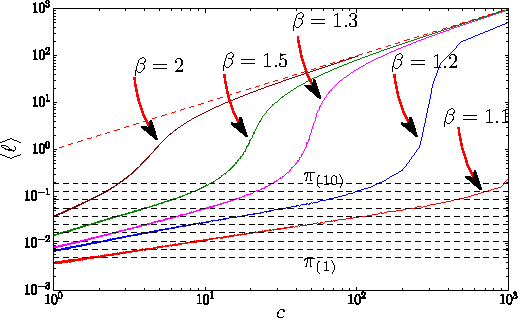
\includegraphics[width=0.8\textwidth]{figs_ineq/cropping-liquidity_global-crop.pdf}
\caption{Time averaged cash $\langle \ell_i \rangle$ as a function of wealth $c_i$, from $\beta= 1.1$ to $\beta =2$  for a system of $N=10^5$ agents exchanging $K=10$ classes of goods ($\pi_{(k)}=\pi_{(1)}g^{k-1}$ with $g=1.5$, $\pi_{(1)}=0.005$, $M_k\pi_{(k)}=\Pi/K$ and $C/\Pi=1.2$). The dashed lines indicate the different prices of goods. Agents with $\langle \ell_i \rangle$ below the price of a good typically have not enough cash to buy it. Cash is proportional to wealth for large levels of wealth (see the upper straight red dashed line).}
\label{Fig:K10_classes}
\end{figure}


When the total number of objects per agent is large for any class $k$, we expect that $\lambda_1, ..., \lambda_K \gg 1$, and then the average values of $z_{i,k}$ are close to their most likely values, as in the single good case. This means that, as with the single good case, and agent with wealth $c_i < \lambda_k \pi_k = c^{(k)}$ will be saturated with goods of type $k'\leq k$ and won't be able to afford goods of type $k'' \geq k$. 

The consequence is that the population of agents now splits into $K$ classes, defined by the intervals $c_i \in [c^{(k-1)},c^{(k)}]$, each filled with objects cheaper than $k$ and unable to purchase more expensive ones. This structure into classes can be seen in the computer simulations of Figure \ref{Fig:K10_classes}, where we present the average cash $\langle \ell_i \rangle$ of agents as a function of their initial wealth $c_i$. The horizontal lines denote the prices $\pi_{(k)}$ of the different objects, and the intersections with the horizontal lines define the thresholds $c^{(k)}$.


\begin{figure}
\centering
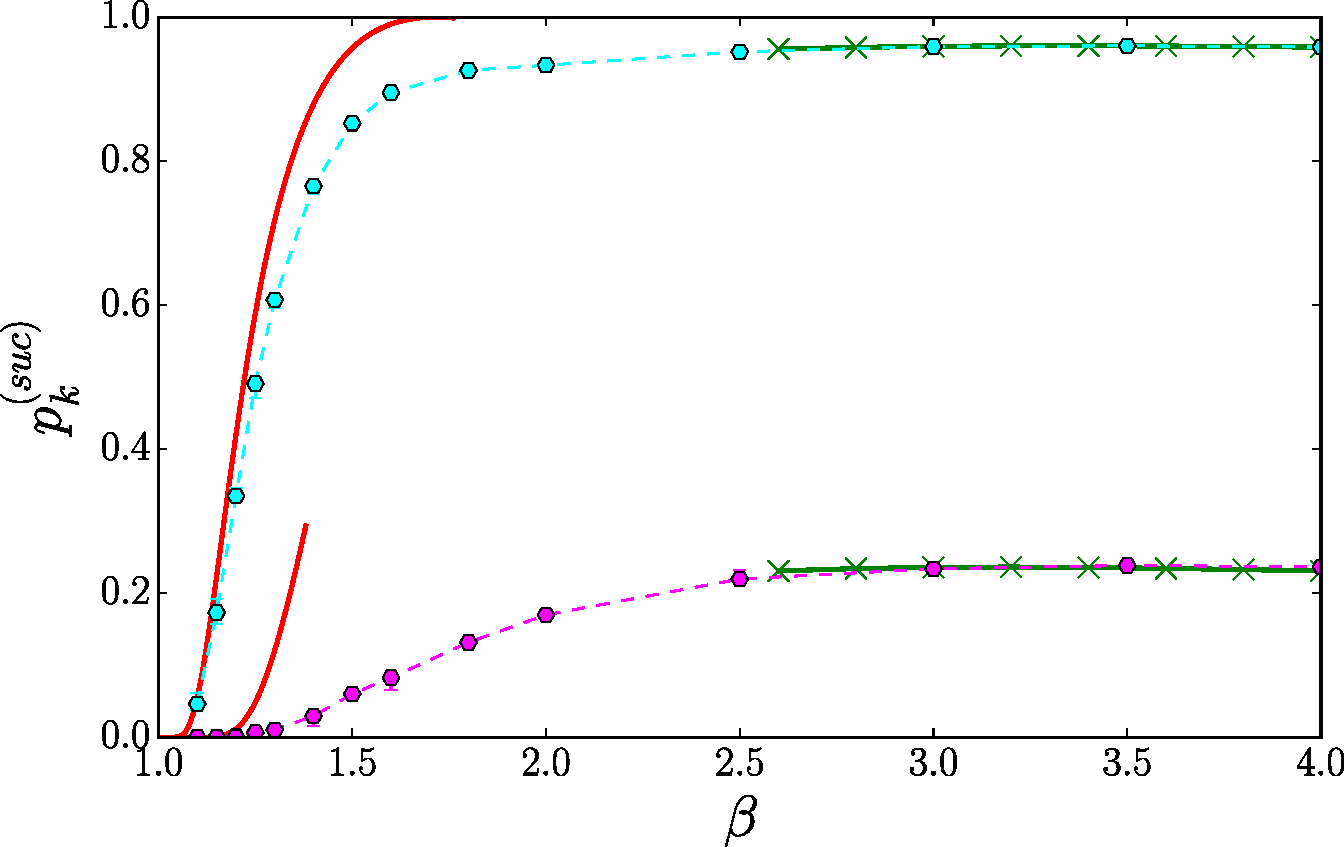
\includegraphics[width=0.8\textwidth]{figs_ineq/fig_K=2_e=1p2_ps_prediction_adjustedcapital.pdf}
\caption{Comparison between numerical simulations and analytical estimates of the success probability of transaction $p^s_k$ for two classes of goods as a function of the Pareto exponent $\beta$. The blue solid circles are the result  of Monte Carlo simulations performed for $N=10^5$ agents and averaged over 5 realizations, with the error bars indicating the min and max value of $p^s_k$ over all realizations. The red lines are the analytic estimates  according to equation \eqref{Eq:ps_and_ck_generalCaseAnyMathcalM1}. The green crossed lines correspond to numerically solving the analytical solution  \eqref{Eq:ME_solution_2Goods} for a population composed of $N=64$ agents.}
\label{Fig:summary_section_one_object}
\end{figure}

To see the effect of inequality in the trade activity, we must again find an analytical expression for the liquidities $p^s$, which are given by the following expression

\begin{equation}
p^s_{k} = 1 - \frac{1}{N}\sum_{i=1}^N P\left(z_{i,k}=m_{i,k}(z_i^{(k)})\right) = 1 - \frac{1}{N}\sum_{i=1}^N P_i(\text{not accepting good type k})
\label{eq:psk_sum}
\end{equation}

An analytic derivation for the $p_k^s$ and $c^{(k)}$ can be obtained only in the limit in which prices are well separated (i.e. $\pi_{(k+1)} \gg \pi_{(k)}$) and the total values of good of any class is approximately constant (we use $M_k\pi_{(k)}  = \Pi / K = {\rm const}$), because in this limit we expect to find a sharp separation of the population of agents into classes. When the prices are separated by an order of magnitude, then $M_1\gg M_2\gg \ldots \gg M_K$, which implies that the market is flooded with objects of the class $1$, which constantly change hands and essentially follow the laws found in the single type of object case. On top of this dense gas of objects of class $1$, we can consider objects of class $2$ as a perturbation (they are picked $M_2/M_1$ times less often). On the time scale of the dynamics of objects of type $2$, the distribution of cash is such that all agents with a wealth less than $c^{(1)}=\pi_{(1)}\lambda_1$ have their budget saturated by objects of type $1$ and typically do not have enough cash to buy objects of type $2$ nor more expensive ones. 
Likewise, there is a class of agents with $c^{(1)}<c_i\le c^{(2)}$ that will manage to afford goods of types $1$ and $2$, but will hardly ever hold goods more expensive that $\pi_{(2)}$, and so on. In this scenario we can write the probability of not accepting a good of type $k$ for an agent in the same linear fashion as in equation \eqref{eq:k1_saturated_prob} for $K=1$:

\begin{align}
P_i(\text{not accepting good type k}) = 
\begin{cases}
1 & \text{ for } m_i \leq \lambda_{k-1} \\
\left( 1 - \frac{m_i}{\lambda_k} \right) & \text{ for } \lambda_{k-1} < m_i < \lambda_k \\
0 & \text{ for } m_i \geq \lambda_k
\end{cases},
\end{align}

Then $p^s_k$ becomes a simple integral by employing the same steps taken on equations \eqref{eq:ps_first_approx}-\eqref{eq:app_ps_analytic1}.

\begin{equation}
p^s_{k} \simeq 1 - \int_{1}^{c^{(k-1)}} dc\, \beta c^{-\beta - 1} - \int_{c^{(k-1)}}^{c^{(k)}} dc\, \beta c^{-\beta - 1} \left( 1 - \frac{c}{c^{(k)}} \right) 
\end{equation}

In the $K$ goods case we now again replace $\frac{M}{N}$ by its average $\frac{\Pi}{C}\frac{\beta}{\beta - 1}\frac{1}{\pi}$ to find, from the definition of $\lambda_k$:

\begin{equation}
p_k^s = \frac{M_k}{N \lambda_k} = \frac{\Pi}{K C} \frac{\langle c \rangle}{c^{(k)}}
\end{equation}

Plugging this back again on the integral above, we get the general recurrence relation for $k$ goods.

\begin{equation}
c^{(k)} = \left(\beta \left( c^{(k-1)} \right)^{1-\beta} - \beta \frac{\Pi}{K C} \right)^{\frac{1}{1-\beta}}.
\end{equation}

Iterating, we write it as a function of the intensive variables 

\begin{equation}
c^{(k)} = \left[ \beta^k  - \left( \frac{\beta - \beta^{k+1}}{1-\beta} \right) \frac{\Pi}{K C} \right] ^{\frac{1}{1-\beta}},
\label{Eq:ps_and_ck_generalCaseAnyMathcalM1}
\end{equation}
 
And finally $p^s_k$ as a function of the intensive variables:

\begin{equation}
p_k^s = \frac{M_k}{N \lambda_k} \simeq \frac{\Pi}{K C} \frac{\langle c \rangle}{c^{(k)}}.
 \label{Eq:ps_and_ck_generalCaseAnyMathcalM2}
\end{equation}


\begin{figure}
\centering
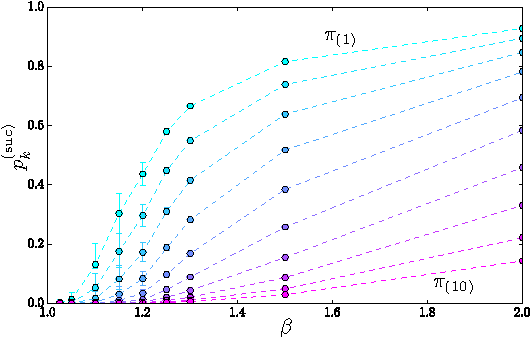
\includegraphics[width=0.8\textwidth]{figs_ineq/cropping-K=10_e=1p2_g=1p5_ps_prediction_adjustedcapital-crop.pdf}
\caption{Liquidity of goods $\{p^s_k\}_{k=1}^K$  as a function of the inequality exponent $\beta$ for a system of $N=10^5$ agents exchanging $K=10$ classes of goods, with parameters $\pi_{(k)}=\pi_{(1)}g^{k-1}$ with $g=1.5$, $\pi_{(1)}=0.005$, $M_k\pi_{(k)}=\Pi/K$ and $C/\Pi=1.2$. Note that all success rates $p^s_k$ vanish when $\beta \to 1^+$.  The curves are ordered from the cheapest good (top) to the most expensive (bottom). The markers are the result of numerical simulations, with error bars indicating the minimum and maximum values obtained by averaging over 5 realizations of the wealth allocations.}
\label{Fig:K10_ps_beta}
\end{figure}

In the limit  $\beta \to 1^+$ of large inequality, close inspection\footnote{Note that the term in square brackets is smaller than one, when $\beta \to 1^+$.} of equation \eqref{Eq:ps_and_ck_generalCaseAnyMathcalM1} shows that $ c^{(k)}  \to \infty, \forall k$, 
which implies that all agents become cash-starved except for the wealthiest few. Since $p^s_{k}\sim \langle c \rangle /c^{(k)}$, this implies that all markets freeze: $p^s_{k}\to 0 , \forall k$.  The arrest of the flow of goods appears to be  extremely robust against all choices of the parameter $\pi_{(k)}$, as $p^s_{1}$ is an upper bound for the other success rates of transactions $p^s_{k}$. These conclusions are fully consistent with the results of extensive numerical simulations, as illustrated in figure \ref{Fig:K10_ps_beta}, in which we simulate an economy with $K=10$ classes of goods (see figure caption for details) and different values of $\beta$. As expected, for a fixed value of the Pareto exponent $\beta$ the success rate increases as the goods become cheaper, as they are easier to trade.  It also shows that trades of all classes of goods halt as $\beta$ tends to unity, which is when wealth inequality becomes too large, independently of their price.


An alternative way to interpret the freezing of the economy is to compare the cash and capital inequalities via their Gini coefficients. The Gini coefficient is a measure of inequality in a distribution: it is a function of the relative mean of the absolute difference among all the elements of the distribution, that is

\begin{equation}
G(\{x_i\}) = \frac{\sum_{i=1}^N \sum_{j=1}^N \| x_i - x_j \|}{2 N \sum_{i=1}^N x_i}
\end{equation}

The normalization term is so that the Gini coefficient has a support on $[0, 1]$ independent of the distribution, and it is invariant to scalings of the type $x_i \to \lambda x_i$. The measure is most commonly used in Economics, for measuring income inequality among different countries, and a Gini coefficient of $0$ means perfect equality, where every point in a distribution is the same, whereas a Gini coefficient close to 1 means perfect inequality: only one point of the (presumed large) distribution is nonzero. 

\begin{figure}[ht]
\centering
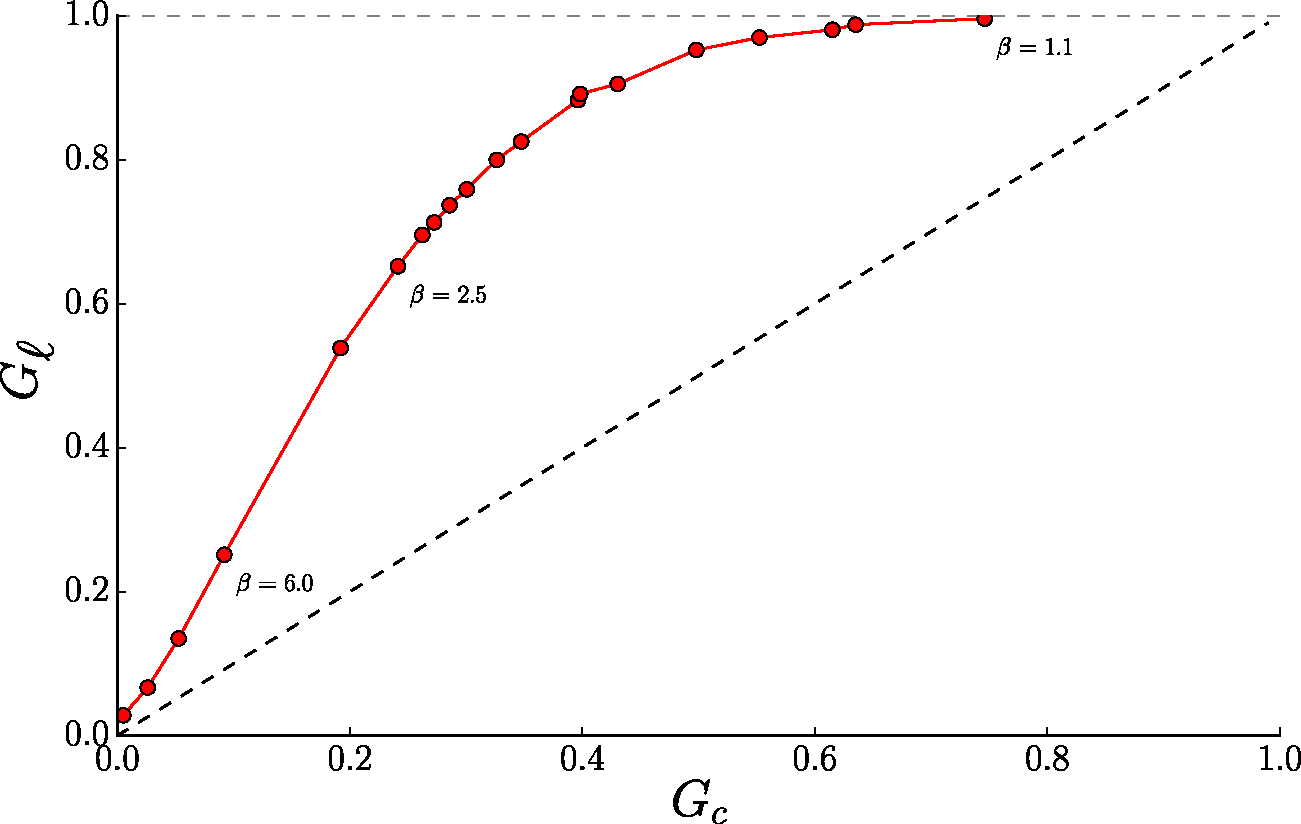
\includegraphics[width=0.75\textwidth]{figs_ineq/gini_intro.pdf}
\caption{Gini coefficient $G_\ell$ of the cash distribution (liquid capital) in the stationary state as a function of the Gini $G_c$ of the wealth distribution, calculated through the numeral simulations of figure \ref{Fig:K10_ps_beta}. The dashed line indicates proportionality between cash and wealth, in which case the inequality in both is the same.}
\label{fig:gini}
\end{figure}

For our economy, we plot on figure \ref{fig:gini} for various values of $\beta$ the Gini coefficient for cash $G_\ell$ as a function of the Gini coefficient for the capital $G_c$ in the $K=10$ system of figure \ref{Fig:K10_ps_beta}. The dashed line is the case where a certain inequality of capital implies the exact same inequality of cash. We see that the liquidity over concentrates, being much more unequal than the original capital distribution, approaching perfect inequality, i.e., concentrating in the hands of few agents much faster than the capital.


Note finally that $p^s_k$ quantifies liquidity in terms of goods. In order to have an equivalent measure in terms of cash that can be compared to the velocity of money described in the Introduction, we average $\pi_{(k)} p^s_k$ over all goods

\begin{equation}
\label{def:pavg}
\bar p^s=\frac{1}{\Pi}\sum_{k=1}^K M_k \pi_{(k)} p^s_k.
\end{equation}

This quantifies the frequency with which a unit of cash changes hand in our model economy as a result of a successful transaction. It's behaviour as a function of $\beta$ for the same parameters of the economy in Figure \ref{Fig:K10_ps_beta} is shown on Figure \ref{fig:data_model}. Even though we cannot make a one to one comparison with real world data, we see that the freezing we observe in the model due to high inequality is, at least qualitatively, corroborated by the data.


\begin{figure}%[htbp]
\centering
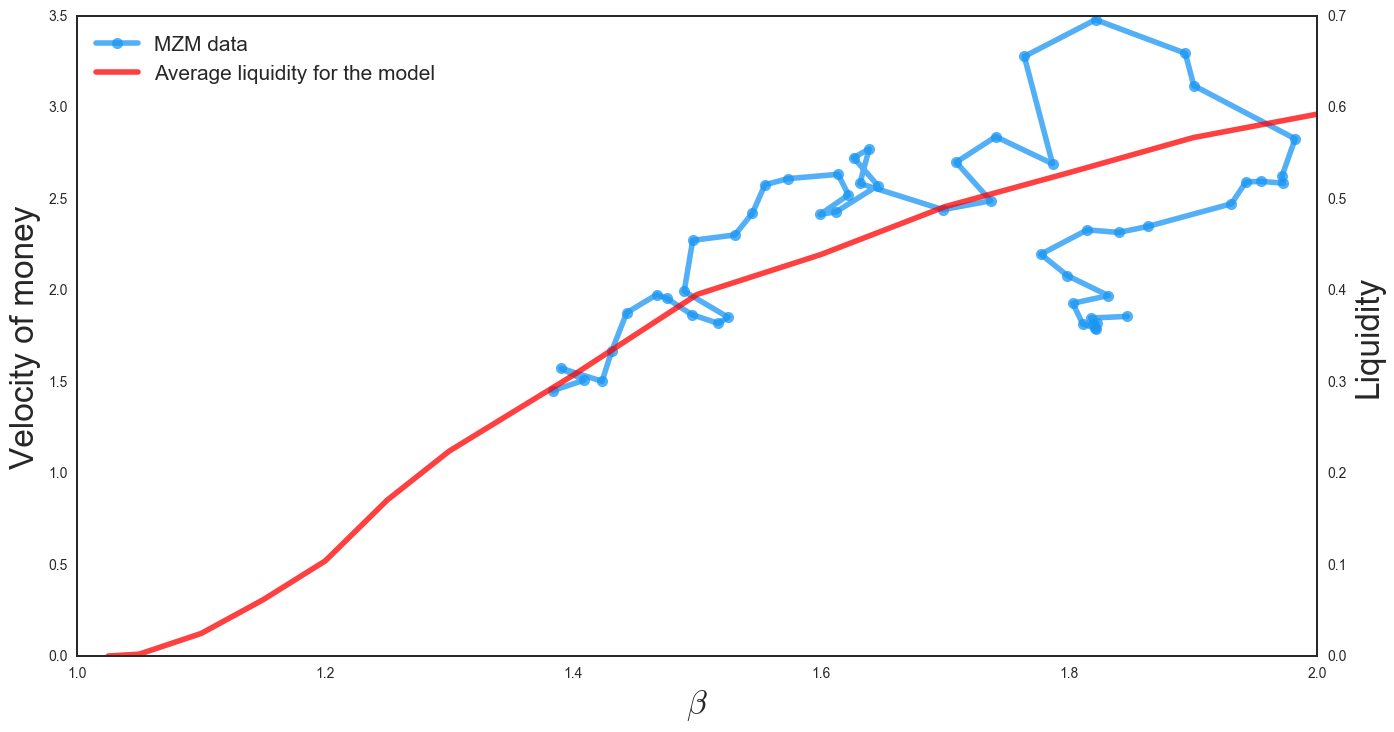
\includegraphics[width=0.8\textwidth]{figs_ineq/data_model.png}
\caption{Comparison of MZM money velocity from the US data to average liquidity (as defined in equation \eqref{def:pavg}) calculated in the simulations of figure \ref{Fig:K10_ps_beta}.}
\label{fig:data_model}
\end{figure}

\section{Conclusions}
\label{sec:con}

We have introduced in this chapter a zero-intelligence trading dynamics in which agents have a Pareto distributed wealth and randomly trade goods with different prices. We have shown that this dynamics leads to a uniform distribution in the space of the allocations that are compatible with the budget constraints and when the inequality in the distribution of wealth increases, the economy converges to an equilibrium where typically (i.e. with probability very close to one) the less wealthy agents have less and less cash available, as their budget becomes saturated by objects of the cheapest type. At the same time this class of cash-starved agents takes up a larger and larger fraction of the economy, thereby leading to a complete halt of the economy when the distribution of wealth becomes so broad that its expected average diverges (i.e. when $\beta \to 1^{+}$). In these cases, a finite number of the wealthiest agents own almost all the cash of the economy. 

The model presented is intentionally simple, so as to highlight a robust and quantifiable link between inequality and liquidity. In particular, the model neglects important aspects such as {\em i)} agents' incentives and preferential trading, {\em ii)} endogenous price dynamics and {\em iii)} credit. It is worth discussing each of these issues in order to address whether the inclusion of some of these factors would revert our finding that inequality and liquidity are negatively related. 

First, our model assumes that all exchanges that are compatible with budget constraints will take place, but in a more realistic setting only exchanges that increase each party's utility should take place, just as we have approached in the rest of this thesis. Yet if the economy freezes in the case where agents would accept all exchanges that are compatible with their budget, it should also freeze when only a subset of these exchanges are feasible. The model also assumes that all agents trade with the same frequency whereas one might expect that rich agents trade more frequently than poorer ones. Could liquidity be restored if trading patterns exhibit some level of homophily, with rich people trading more often and preferentially with rich people? 

First we note that both these effects are already present in our simple setting. Agents with higher wealth are selected more frequently as sellers as they own a larger share of the objects. In spite of the fact that buyers are chosen at random, successful trades occur more frequently when the buyer is wealthy. So, in the trades actually observed the wealthier do trade more frequently than the less wealthy, and preferentially with other wealthy agents. Furthermore, if agents are allowed to trade only with agents having a similar wealth (e.g. with the $q$ agents immediately wealthier or less wealthy) it is easy to show that detailed balance still holds with the same uniform distribution on allocations. As long as all the states are accessible, the stationary probability distribution remains the same: the dynamics would change and thus $p_k^s$ would too change, in particular for goods more expensive than $\pi_{(1)}$, the seller is typically cash-rich and thus its neighbours are too. This can induce to have a liquidity of expensive goods higher than that of cheaper ones. However in the limit $\beta \to 1^{+}$, it is still true that cash concentrates in the hands of a vanishing fraction of agents, and there is still a freeze of the economy. Therefore, the model conclusions are robust with respect to a wide range of changes in its basic setting that would account for more realistic trading patterns. 

Secondly, it is reasonable to expect that prices will adjust -- i.e. deflate -- as a result of a diminished demand caused by the lack of liquidity. Within the model, the inclusion of price adjustment, occurring on a slower time-scale than trading activity, would reduce the ratio $\Pi/C$ (between total value of goods and total wealth), but it would also change the wealth distribution. Since the freezing phase transition occurs irrespective of the ratio $\Pi/C$, the first effect, though it might alleviate the problem, would not change the main conclusion. The second effect would make it more compelling, because cash would not depreciate as prices do, so deflation would leave 
wealthy agents -- who hold most of the cash -- even richer compared to the cash deprived agents, that would suffer the most from deflation. So while price adjustment apparently increases liquidity, this may promote further inequality, which would curtail liquidity further. 

Finally, can the liquidity freeze be avoided by allowing agents to borrow? Access to credit will hardly improve the situation. Allowing agents to borrow using goods as collaterals is equivalent to doubling the
wealth of cash-starved agents, provided that any good can be used only once as a collateral, and that goods bought with credit cannot themselves be used as collaterals.  This would at most blur the crossover between cash-rich agents and cash-starved ones, as intermediate agents would sometimes use credit. This does not change the main conclusion that inequality and liquidity are inversely related and that the economy would halt when $\beta \to 1^{+}$. This is in line with the results in \cite{Yakovenko2009Review} and for similar reasons. Credit may mitigate illiquidity in the short term, but cash deprived agents would have to borrow from wealthier ones. With positive interest rates, this would make inequality even larger in the long run. Credit is therefore likely to make things worse, in line with the arguments\footnote{Piketty \cite{Piketty2014} observes that when the rate of return on capital exceeds the growth rate of the economy (which is zero in our setting), wealth concentrates more in the hands of the rich.} in \cite{Piketty2014}.

Therefore, even though the model presented here can be enriched in many ways, it's not clear what would revert the relation between inequality and liquidity. 

Corroborating the present model with empirical data goes beyond the scope of this work, yet we remark that our findings are consistent with recent economic trends, as shown in Figure \ref{Fig:data}.  For example, it is worth observing that, alongside with increasing levels of inequality, trade 
has slowed down after the 2008 crisis\footnote{The {\em U.S. Trade Overview, 2013} of the International Trade Administration observes that ``Historically, exports have grown as a share of U.S. GDP. However, in 2013 exports contributed to 13.5\% of U.S. GDP, a slight drop from 2012'" (see {\tt http://trade.gov/mas/ian/tradestatistics/index.asp{\#P}11}). A similar slowing down can be observed at the global level, in the UNCTAD {\em Trade and Development Report, 2015}, page 7 (see {\tt http://unctad.org/en/pages/PublicationWebflyer.aspx?publicationid=1358}).}. More generally, avoiding deflation, or promoting inflation,  has been a major target of monetary policies after 2008, which one could take as an indirect evidence of the slowing down of the economy.  Furthermore, the fact that inequality hampers liquidity and hence promotes demand for credit suggests that the boom in credit market before 2008 and the increasing levels of inequality might not have been a coincidence. 

An interesting side note is that the concentration of capital in the top agents goes hand in hand with a flow of cash to the top. Indeed, in the model an injection of extra capital in the lower part of the wealth pyramid --the so-called {\em helicopter money} policy-- is necessarily followed by a flow of this extra cash to the top, via many intermediate agents, thus generating many transactions on the way. This \textit{trickle up} dynamics should be contrasted with the usual idea of the \textit{trickle down} policy, which advocates injections of money to the top in order to boost investment. In this respect, it is tempting to relate our findings to the recent debate on Quantitative Easing measures, and in particular to the proposal that the (European) central bank should finance households (or small businesses) rather than financial institutions in order to stimulate the economy and raise inflation \cite{QEvox,QEft}. Clearly, our results support the helicopter money policy, because injecting cash at the top does not disengages the economy from a liquidity stall. 

Extending our minimal model to take into account the endogenous dynamics of the wealth distribution and of prices, accounting for investment and credit, is an interesting avenue of future research, for which the present work sets the stage. In particular, this could shed light on understanding the conditions under which the positive feedback between returns on investment and inequality, that lies at the very core of the dynamics which has produced ever increasing levels of inequality according to \cite{Piketty2001,Piketty2014,SaezZucman2016}, sets in.